\documentclass[12pt]{article}
\usepackage[a4paper,margin=1.25cm]{geometry}
\usepackage{amsmath,amssymb,mathtools}
\usepackage{graphicx}
\usepackage{booktabs}
\usepackage{tabularx}
\usepackage{tikz}
\usepackage[T1]{fontenc}
\usepackage[utf8]{inputenc}
\usepackage[english]{babel}

\setlength{\parindent}{0pt}
\setlength{\parskip}{0.45em}
\setlength{\abovedisplayskip}{5pt plus 1pt minus 1pt}
\setlength{\belowdisplayskip}{5pt plus 1pt minus 1pt}
\setlength{\abovedisplayshortskip}{3pt plus 1pt minus 1pt}
\setlength{\belowdisplayshortskip}{3pt plus 1pt minus 1pt}

\newcommand{\dd}{\,\mathrm{d}}
\newcommand{\e}{\mathrm{e}}
\newcommand{\Mid}{m}

\begin{document}

\begin{center}
{\Large\bfseries A geometric mean beats the logarithm}\\[0.35em]
{\large \(\displaystyle\int_k^{k+1}\frac{\mathrm dx}{x}<\frac1{\sqrt{k(k+1)}}\), term by term}
\end{center}

\[
\boxed{\displaystyle
\frac1{\sqrt{1^2+1}}+\frac1{\sqrt{2^2+2}}+\cdots+\frac1{\sqrt{n^2+n}}
>\log(n+1),\qquad n\ge1 .}
\]

\textbf{Overview.}
Both sides telescope into \(n\) matching pieces. On the right,
\[
\log(n+1)=\sum_{k=1}^{n}\log\frac{k+1}{k}
=\sum_{k=1}^{n}\int_k^{k+1}\frac{\dd x}{x},
\]
and on the left the \(k\)-th term is the integral of the constant
\(\frac1{\Mid}\) over the same interval, where
\[
\Mid=\sqrt{k(k+1)}=\sqrt{k^2+k}
\]
is the geometric mean of the endpoints. So the whole inequality follows
from the single statement
\[
\int_k^{k+1}\frac{\dd x}{x}<\frac1{\Mid},
\qquad \Mid=\sqrt{k(k+1)} .
\tag{$\ast$}
\]
This is a strict comparison between the average of \(\frac1x\) on
\([k,k+1]\) and its value at the geometric mean of the endpoints.
Convexity is not enough: it compares with the \emph{arithmetic} mean and
yields the inequality in the useless direction. It follows instead from the reflection symmetry
\(x\mapsto\Mid^2/x\), which is exactly the symmetry fixing the geometric
mean.

Two proofs of \((\ast)\) are given: one by the reflection, and one by a
change of variable that reduces it to the classical
\(2\log s<s-\frac1s\).

\section*{1. Reduction to a single interval}

Telescoping the logarithm,
\[
\log(n+1)=\log\frac21+\log\frac32+\cdots+\log\frac{n+1}{n}
=\sum_{k=1}^{n}\int_k^{k+1}\frac{\dd x}{x} .
\tag{1}
\]
Since \(\Mid=\sqrt{k(k+1)}\) is a constant on \([k,k+1]\),
\[
\frac1{\sqrt{k^2+k}}=\int_k^{k+1}\frac{\dd x}{\Mid} .
\tag{2}
\]
So the difference of the two sides of the problem is
\[
\sum_{k=1}^{n}\int_k^{k+1}\left(\frac1{\Mid}-\frac1x\right)\dd x ,
\]
and it suffices to prove that each summand is positive, i.e. \((\ast)\).

\section*{2. First proof: reflect about the geometric mean}

Fix \(k\ge1\) and \(\Mid=\sqrt{k(k+1)}\). By AM--GM,
\(k<\Mid<k+1\), so the integrand \(\frac1{\Mid}-\frac1x\) changes sign
exactly once, at \(x=\Mid\): it is negative on \([k,\Mid)\) and positive
on \((\Mid,k+1]\). Write
\[
\int_k^{k+1}\left(\frac1{\Mid}-\frac1x\right)\dd x
=-\underbrace{\int_k^{\Mid}\left(\frac1x-\frac1{\Mid}\right)\dd x}_{S_-}
+\underbrace{\int_{\Mid}^{k+1}\left(\frac1{\Mid}-\frac1x\right)\dd x}_{S_+},
\tag{3}
\]
with \(S_\pm>0\). The claim is \(S_+>S_-\).

The decisive observation is that the involution
\[
x\longmapsto\frac{\Mid^2}{x}
\]
maps \([k,\Mid]\) onto \([\Mid,k+1]\), because
\(\frac{\Mid^2}{k}=\frac{k(k+1)}{k}=k+1\). This is the only place where
the choice \(\Mid=\sqrt{k(k+1)}\) is used, and it is the reason that
choice is forced.

Substituting \(x=\Mid^2/t\), \(\dd x=-\frac{\Mid^2}{t^2}\dd t\), in
\(S_-\):
\[
\left(\frac1x-\frac1{\Mid}\right)\dd x
=\left(\frac{t}{\Mid^2}-\frac1{\Mid}\right)\left(-\frac{\Mid^2}{t^2}\right)\dd t
\quad\longrightarrow\quad
S_-=\int_{\Mid}^{k+1}\frac{t-\Mid}{t^2}\dd t .
\tag{4}
\]
Meanwhile
\[
S_+=\int_{\Mid}^{k+1}\frac{x-\Mid}{\Mid x}\dd x .
\tag{5}
\]
Both integrals are now over the \emph{same} interval, so they can be
subtracted pointwise:
\[
S_+-S_-
=\int_{\Mid}^{k+1}(x-\Mid)\left(\frac1{\Mid x}-\frac1{x^2}\right)\dd x
=\int_{\Mid}^{k+1}\frac{(x-\Mid)^2}{\Mid\,x^2}\dd x>0 .
\tag{6}
\]
The integrand is a perfect square divided by positive quantities, and it
is not identically zero. Hence \((\ast)\) holds strictly.

\begin{center}
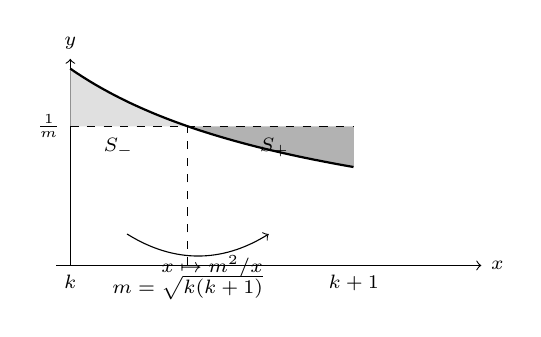
\begin{tikzpicture}[x=3.6cm,y=2.5cm]
\draw[->] (0.95,0)--(2.45,0) node[right] {\scriptsize \(x\)};
\draw[->] (1.0,0)--(1.0,1.05) node[above] {\scriptsize \(y\)};
\def\ka{1.0}
\def\kb{2.0}
\pgfmathsetmacro{\mg}{sqrt(2)}
\pgfmathsetmacro{\ym}{1/sqrt(2)}
\fill[black!12] plot[domain=1.0:1.41421,samples=60] (\x,{1/\x}) -- (1.41421,\ym) -- (1.0,\ym) -- cycle;
\fill[black!30] (1.41421,\ym) -- (2.0,\ym) -- plot[domain=2.0:1.41421,samples=60] (\x,{1/\x}) -- cycle;
\draw[thick,samples=140,domain=1.0:2.0,smooth] plot (\x,{1/\x});
\draw[dashed] (1.0,\ym)--(2.0,\ym);
\draw[dashed] (1.41421,0)--(1.41421,\ym);
\node[below] at (1.0,0) {\scriptsize \(k\)};
\node[below] at (2.0,0) {\scriptsize \(k+1\)};
\node[below] at (1.41421,0) {\scriptsize \(\Mid=\sqrt{k(k+1)}\)};
\node[left] at (1.0,\ym) {\scriptsize \(\tfrac1{\Mid}\)};
\node at (1.17,0.60) {\scriptsize \(S_-\)};
\node at (1.72,0.60) {\scriptsize \(S_+\)};
\draw[->] (1.20,0.16) to[bend right=32] (1.70,0.16);
\node[anchor=north] at (1.5,0.10) {\scriptsize \(x\mapsto \Mid^2/x\)};
\end{tikzpicture}
\end{center}

\section*{3. Second proof: one substitution}

The inequality \((\ast)\) can also be normalised away entirely. Put
\[
s=\sqrt{\frac{k+1}{k}}>1 .
\]
Then
\[
\int_k^{k+1}\frac{\dd x}{x}=\log\frac{k+1}{k}=2\log s,
\]
and, since \(\frac1k=s^2-1\) and \(\sqrt{k(k+1)}=ks\),
\[
\frac1{\sqrt{k(k+1)}}=\frac1{ks}=\frac{s^2-1}{s}=s-\frac1s .
\]
So \((\ast)\) is precisely
\[
\boxed{\displaystyle 2\log s<s-\frac1s\qquad (s>1).}
\tag{7}
\]
This is immediate: let \(h(s)=s-\frac1s-2\log s\). Then \(h(1)=0\) and
\[
h'(s)=1+\frac1{s^2}-\frac2s=\left(1-\frac1s\right)^2\ge0,
\]
with strict positivity for \(s>1\). Hence \(h(s)>0\) for \(s>1\). \(\square\)

Inequality (7) has independent interest. It states
that \(\log\) grows more slowly than the odd hyperbolic-type function
\(s\mapsto\frac12(s-s^{-1})\), with contact of order three at \(s=1\).
Written with \(s=\e^{u/2}\) it reads \(u<2\sinh\frac u2\), which is the
familiar \(\sinh t>t\).

\section*{4. Conclusion and sharpness}

Summing \((\ast)\) over \(k=1,\dots,n\) and using (1) and (2),
\[
\log(n+1)=\sum_{k=1}^{n}\int_k^{k+1}\frac{\dd x}{x}
<\sum_{k=1}^{n}\frac1{\sqrt{k^2+k}},
\]
which is the assertion.

The inequality is not far from an equality in the following sense. From
(6) the \(k\)-th gap is
\[
\frac1{\sqrt{k^2+k}}-\log\frac{k+1}{k}
=\int_{\Mid}^{k+1}\frac{(x-\Mid)^2}{\Mid x^2}\dd x
=\frac1{24k^3}+O\!\left(\frac1{k^4}\right),
\]
as one checks by expanding both terms in \(\varepsilon=\frac1k\):
\(\frac1{\sqrt{k^2+k}}=\varepsilon-\frac{\varepsilon^2}{2}+\frac{3\varepsilon^3}{8}-\cdots\)
and \(\log(1+\varepsilon)=\varepsilon-\frac{\varepsilon^2}{2}+\frac{\varepsilon^3}{3}-\cdots\),
whose difference starts at \(\bigl(\frac38-\frac13\bigr)\varepsilon^3\).
So the two sides differ by a convergent series and
\[
\sum_{k=1}^{n}\frac1{\sqrt{k^2+k}}-\log(n+1)\longrightarrow c
=0.0190285404\ldots
\]
The excess is a genuine constant, not a growing quantity: the inequality
is asymptotically tight at the level of the leading term \(\log n\).

\begin{center}
\small
\renewcommand{\arraystretch}{1.35}
\begin{tabularx}{0.9\textwidth}{@{}lXXX@{}}
\toprule
\(n\) & \(\sum_{k\le n}(k^2+k)^{-1/2}\) & \(\log(n+1)\) & difference \\
\midrule
\(1\)    & \(0.7071068\) & \(0.6931472\) & \(0.0139596\) \\
\(5\)    & \(1.8102110\) & \(1.7917595\) & \(0.0184517\) \\
\(50\)   & \(3.9508465\) & \(3.9318256\) & \(0.0190205\) \\
\(1000\) & \(6.9277834\) & \(6.9087548\) & \(0.0190285\) \\
\bottomrule
\end{tabularx}
\end{center}

\section*{5. Why the geometric mean, and what fails otherwise}

The natural first attempt is to bound \(\int_k^{k+1}\frac{\dd x}{x}\)
using convexity of \(\frac1x\). The midpoint rule for a convex function
gives
\[
\int_k^{k+1}\frac{\dd x}{x}\ \ge\ \frac1{k+\frac12},
\]
the wrong direction, and indeed \(\frac1{k+1/2}<\frac1{\sqrt{k^2+k}}\)
since \(k+\frac12>\sqrt{k(k+1)}\) by AM--GM. Convexity alone is therefore
not enough; one needs the specific point at which the reflection symmetry
of \(\frac1x\) is centred.

\begin{center}
\small
\renewcommand{\arraystretch}{1.45}
\begin{tabularx}{\textwidth}{@{}>{\raggedright\arraybackslash}p{0.30\textwidth}>{\raggedright\arraybackslash}p{0.24\textwidth}X@{}}
\toprule
Comparison point \(c\in[k,k+1]\) & \(\displaystyle\int_k^{k+1}\frac{\dd x}{x}\) vs \(\frac1c\) & Reason \\
\midrule
\(c=k+\frac12\) (arithmetic mean)
& \(\displaystyle\int>\frac1c\)
& Midpoint rule for a convex function. \\
\addlinespace
\(c=\sqrt{k(k+1)}\) (geometric mean)
& \(\displaystyle\int<\frac1c\)
& Sections 2--3; the map \(x\mapsto c^2/x\) exchanges the two halves. \\
\addlinespace
\(c=\frac{1}{\log\frac{k+1}{k}}\) (logarithmic mean)
& equality
& By definition of the logarithmic mean. \\
\bottomrule
\end{tabularx}
\end{center}

The three rows are the classical chain
\[
\text{harmonic}\le\text{geometric}\le\text{logarithmic}\le\text{arithmetic},
\]
and the problem is exactly the second inequality of that chain applied to
the pair \((k,k+1)\). Seen this way, \((\ast)\) is a standard inequality with a name, and the
reflection proof of Section 2 is the usual proof of \(G\le L\).

\end{document}
